\RequirePackage{plautopatch}

\documentclass[a4paper, 11pt]{ltjsarticle}


% マージン設定
\usepackage[top=20mm, bottom=20mm, left=20mm, right=20mm]{geometry}

% LuaLaTeX用日本語対応パッケージ
\usepackage{luatexja}
\usepackage{luatexja-fontspec}

% 必要なパッケージ
\usepackage{fontspec}
\usepackage{titlesec}
\usepackage{graphicx}
\usepackage{amsmath}
\usepackage{amssymb}
\usepackage[colorlinks=true, linkcolor=black]{hyperref}
\usepackage{tocloft}
\usepackage{indentfirst}
\usepackage{tikz} % カスタム点線用
\usepackage{here}
\usepackage{caption}
\usepackage{bookmark}
\usepackage{multicol}
\usepackage{multirow}
\usepackage{flushend}
\usepackage{subfig}
\usepackage{threeparttable}
\usepackage{enumitem}
\usepackage{url}


\setlength{\baselineskip}{14pt}
\setlength{\parindent}{1\zw}

\titleformat{\section}{\large\bfseries}{\thesection.}{1\zw}{}
\titleformat{\subsection}{\large\bfseries}{\thesubsection.}{1\zw}{}
\titleformat{\subsubsection}{\large\bfseries}{\thesubsubsection.}{1\zw}{}

\setcounter{tocdepth}{3}
\makeatletter
\renewcommand{\numberline}[1]{#1.~}
\renewcommand{\cftsecleader}{\cftdotfill{\cftdotsep}}
\renewcommand{\cftsubsecleader}{\hfill}
\renewcommand{\cftsubsubsecleader}{\hfill}
\cftpagenumbersoff{subsection}
\cftpagenumbersoff{subsubsection}
\makeatother

\DeclareCaptionFont{designatedFont}{\fontsize{11pt}{14pt}\selectfont}
\captionsetup{font=designatedFont}

%---ここから中身---------------------------------------------------------------------------------------
\begin{document}
\fontsize{11pt}{14pt}\selectfont

%---表紙---------------------------------------------------------------------------------------
\thispagestyle{empty}
\begin{center}
\pagenumbering{gobble}  %ページ番号をカウントしない

\vspace*{40mm}
{\huge\noindent 災害時を想定したアドホックネットワーク}\\
\medskip
{\huge\noindent 構築手法の検討}\\
\vspace{\baselineskip}
{\huge\noindent\textbf{Study of Construction Methods for Ad-Hoc Network under Disaster}}\\
\vspace{120mm}

{\huge\noindent
2025年3月4日\\
東京都立産業技術高等専門学校\\
ものづくり工学科 情報通信工学コース \\
末廣 隼人\\
指導教員 髙﨑 和之    \\
}
\vspace{40mm}

\end{center}

%---目次------------------------------------------------------------------------------------------
\clearpage  %新しいページの追加
\thispagestyle{empty}
\tableofcontents  %目次の自動生成 目次をクリックするとその章,節に飛ぶことができる

%---はじめに---------------------------------------------------------------------------------------
\clearpage
\pagenumbering{arabic}
\section{はじめに}
・日本では地震をはじめ多くの自然災害が発生しており,災害時には通信ネットワークが使えなくなる可能性がある.
そこで,アドホックネットワークを活用し地域限定ながら被災状況の把握や情報伝達を可能とする研究が行われている.
・本研究では,人口密度に応じた経路構築方法を考案し,その効果をシミュレーションを用いて検証した.
・近年,Bluetoothの開発が活発に行われており,従来のBluetoothよりも低消費電力で


%---理論---------------------------------------------------------------------------------------
\clearpage
\section{理論}
\subsection{Bluetoothの規格について}
\subsection{アドホックネットワークの技術的課題}
\subsubsection{隠れ端末問題}
隠れ端末問題とは、図1のようにノードAとCがノードBに対して通信を行うとき、ノードAとCはお互いの存在が隠れてしまい、
現在誰も通信を行なってないと思い込んで同時にノードBへと通信を行いデータが衝突してし壊れてしまう問題である。%
\begin{figure}[H]
  \centering
  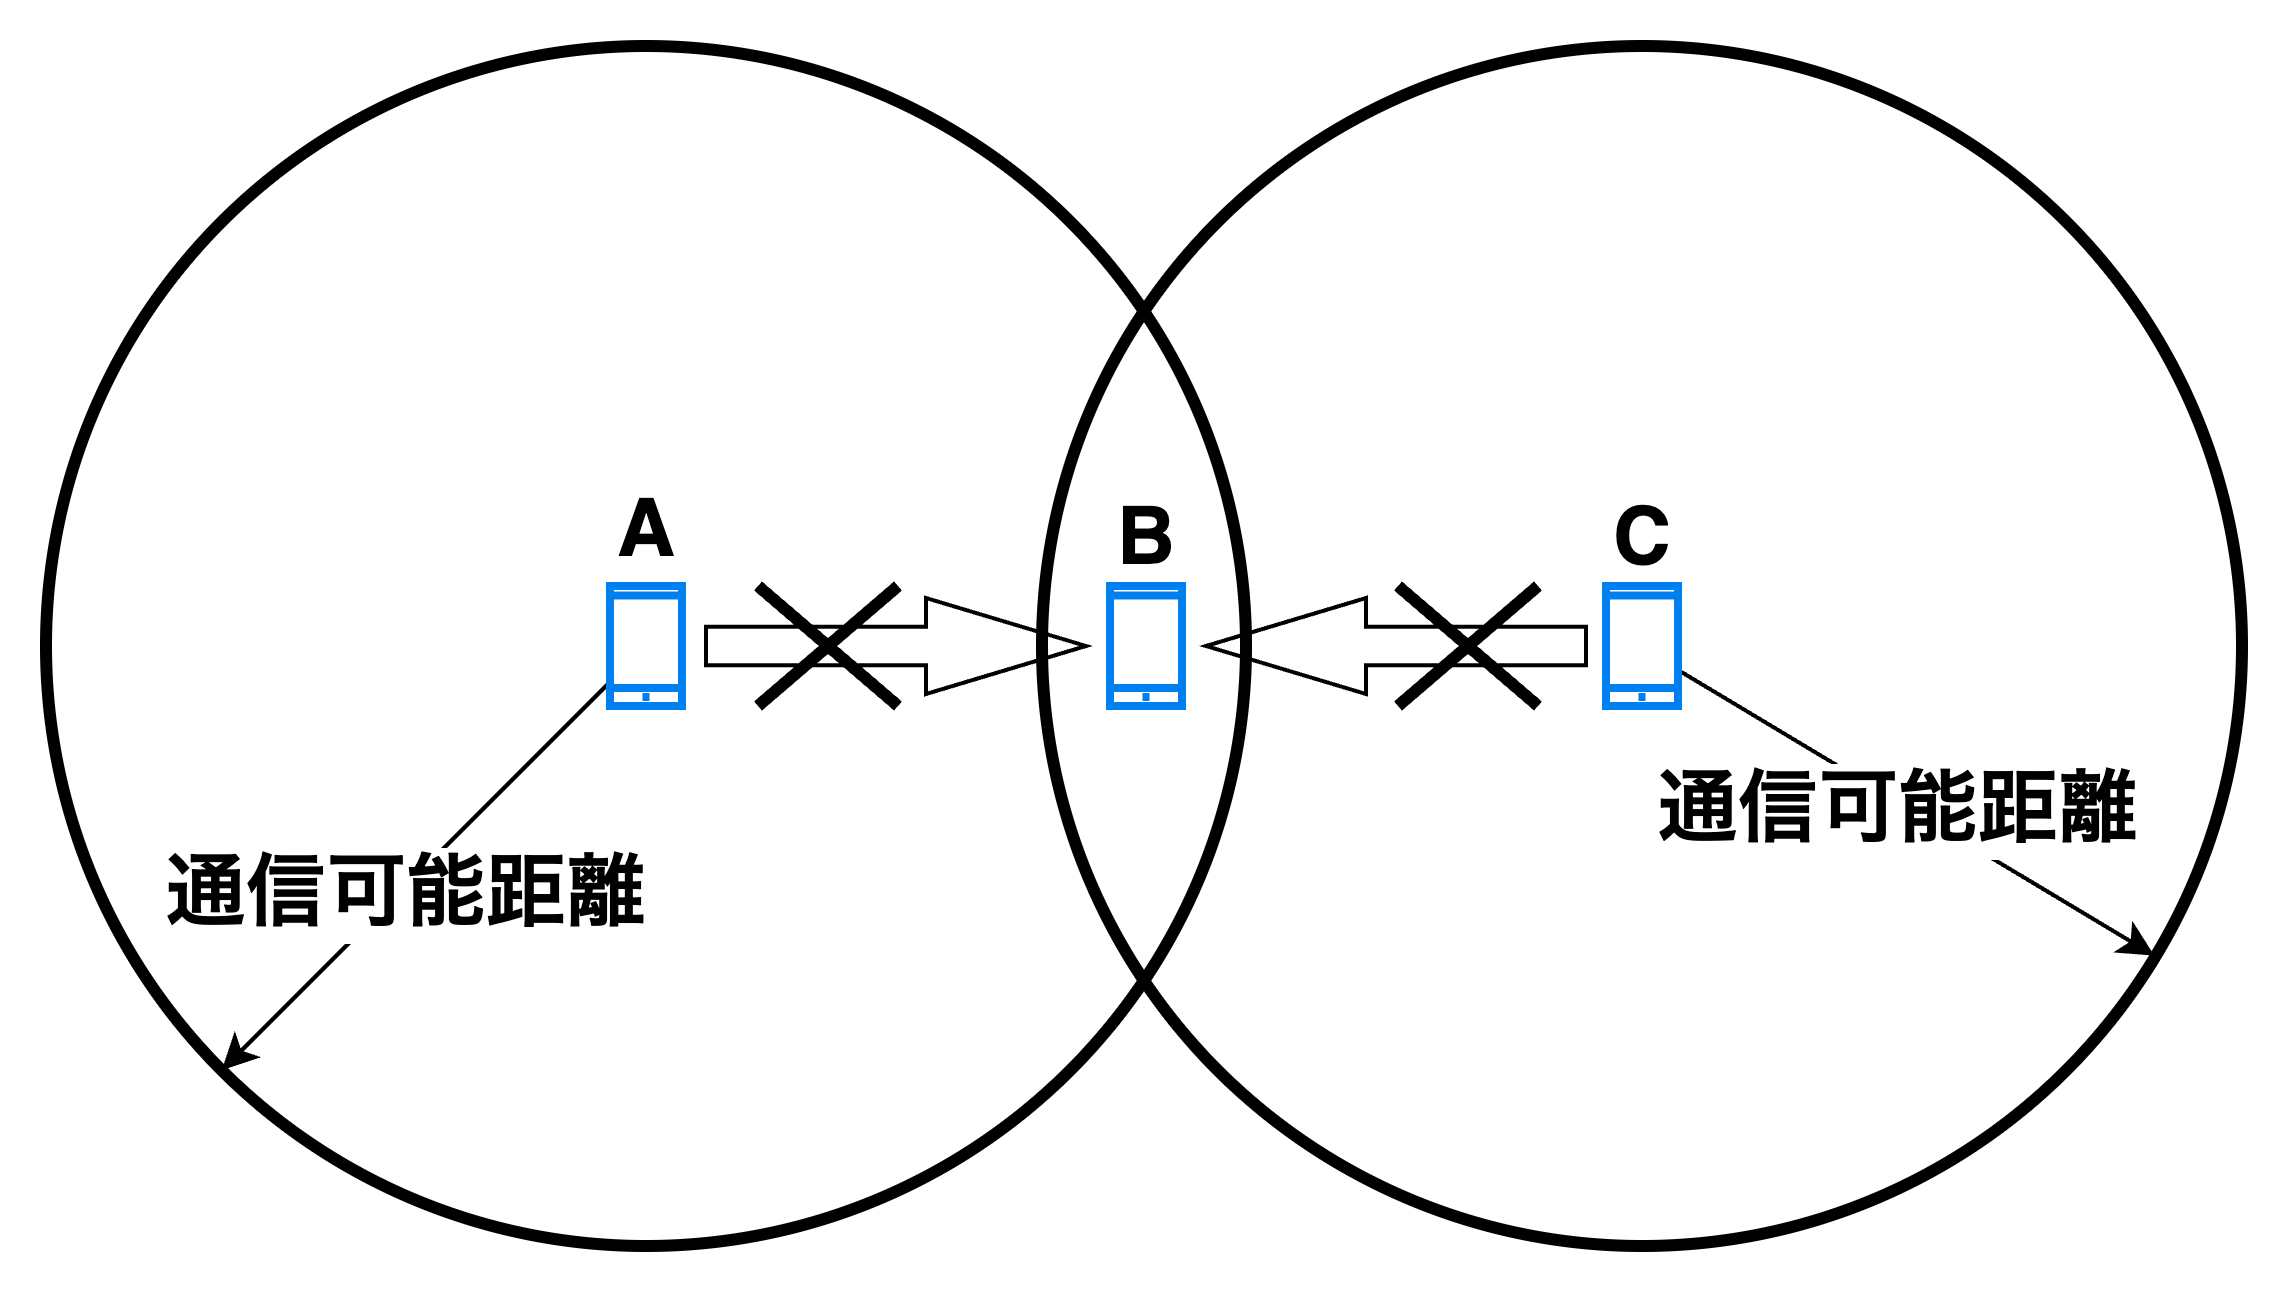
\includegraphics[width=70mm]{hidden_terminal_problem.png}
  \caption{隠れ端末問題}
\end{figure}

\subsubsection{さらし端末問題}
さらし端末問題\cite{人口密度}とは、図2のようにノードAがDと通信を行なっているときノードBは端末Cと通信ができそうだが、
ノードAがDと通信を行なっているため周辺にいる他ノードは通信の抑制がされてしまい、
伝送速度や通信品質の低下が発生してしまう問題である。%
\begin{figure}[H]
  \centering
  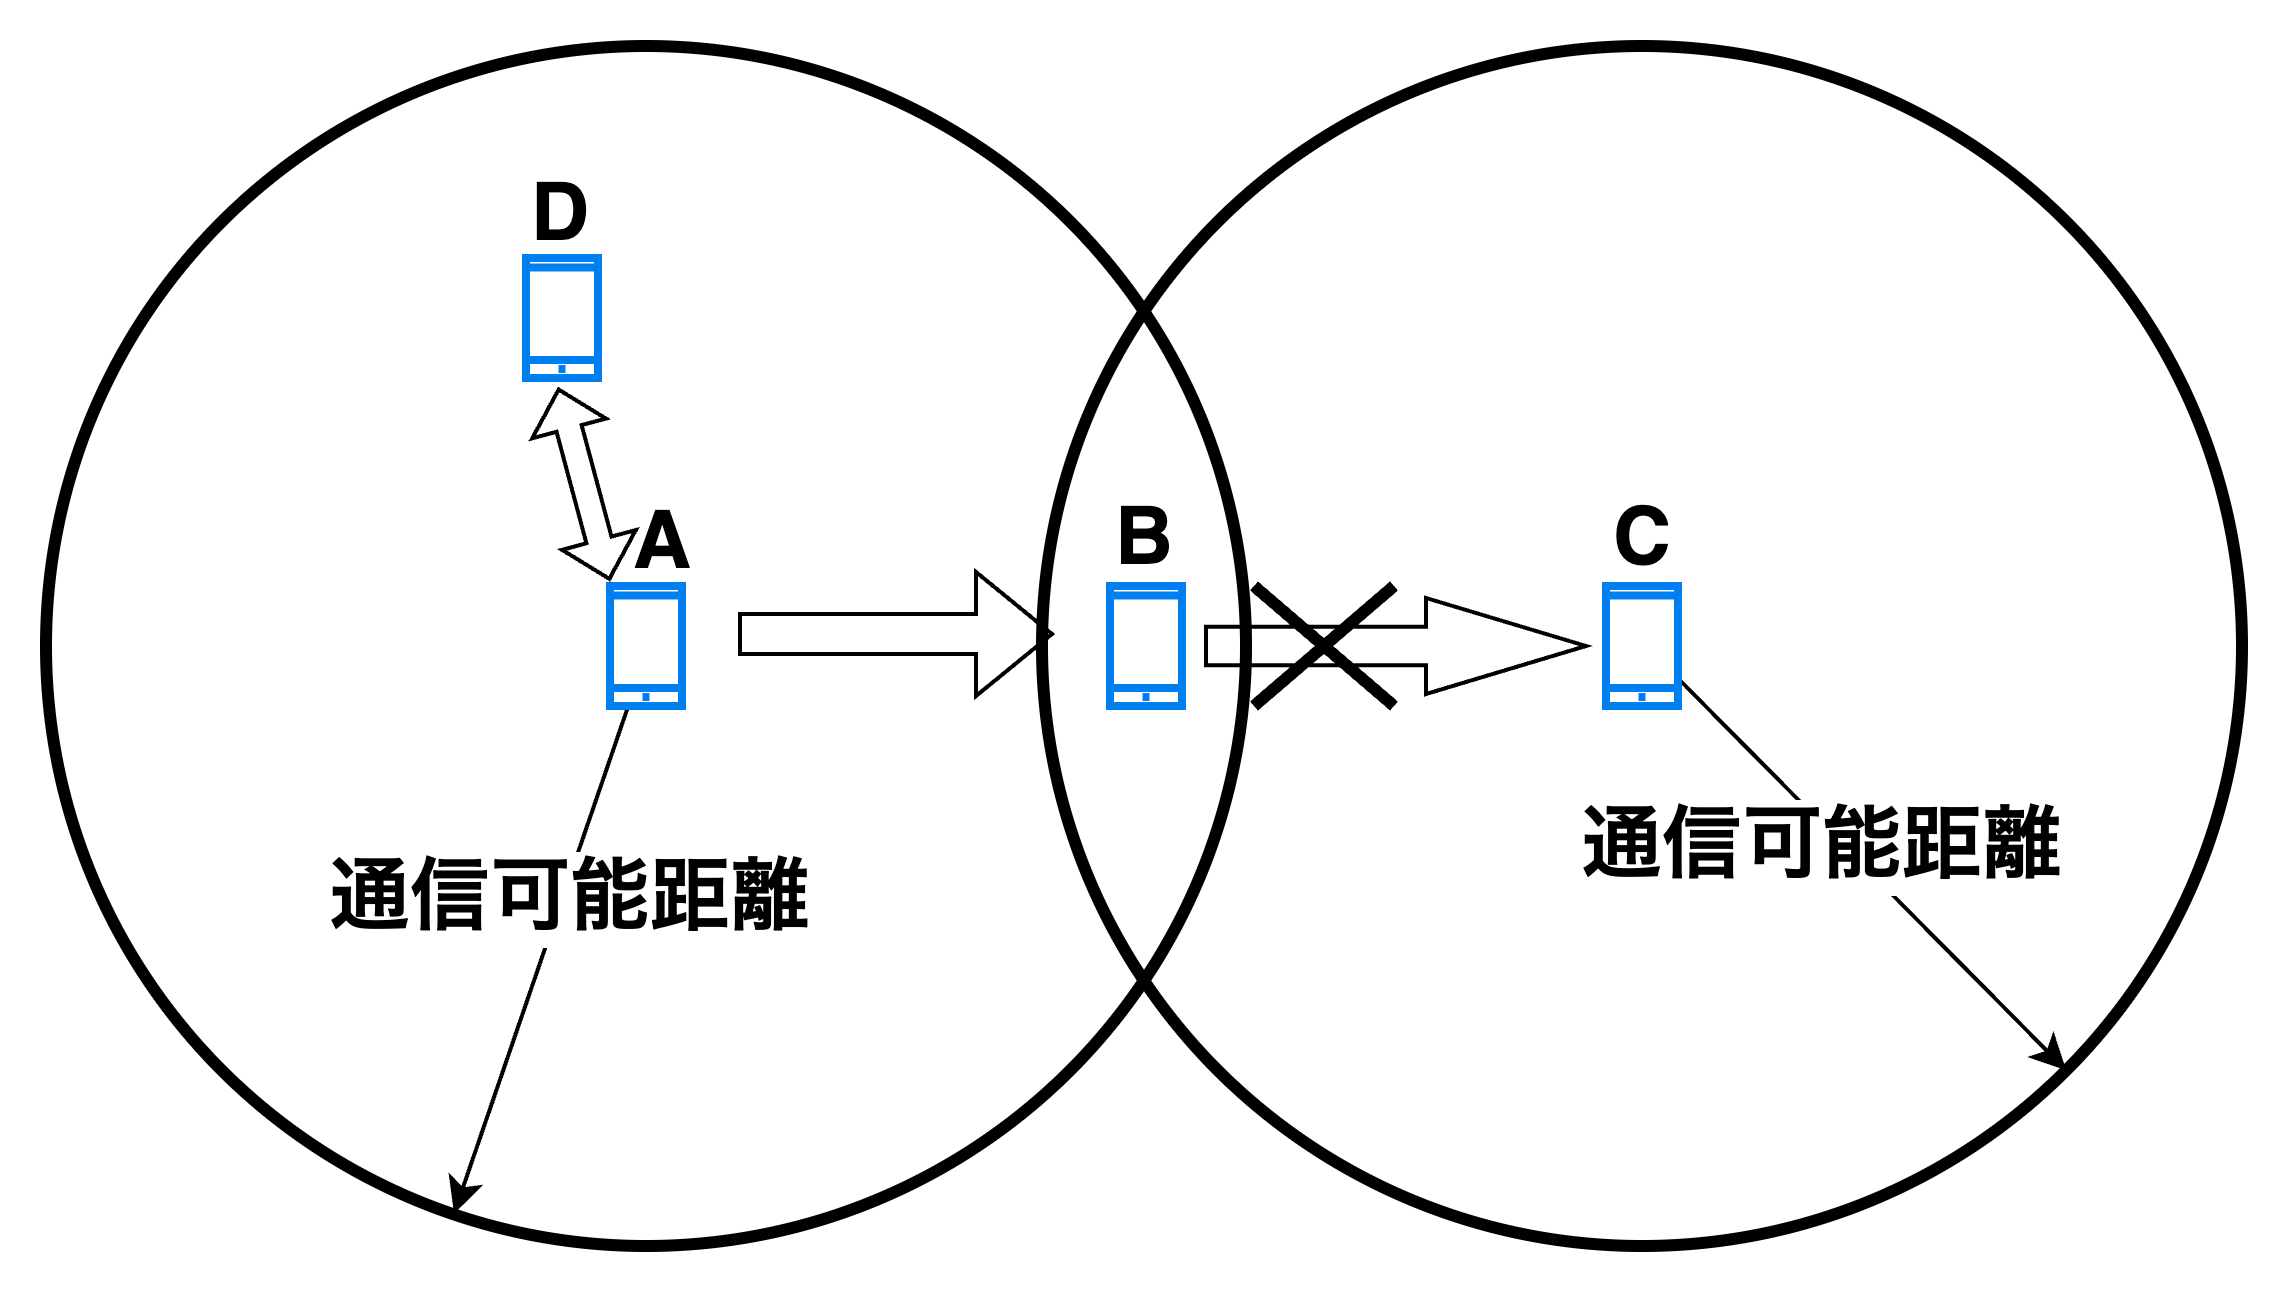
\includegraphics[width=70mm]{exposed_terminal_problem.png}
  \caption{さらし端末問題}
\end{figure}

%---提案手法---------------------------------------------------------------------------------------
\clearpage
\section{提案手法}

%---結果---------------------------------------------------------------------------------------
\clearpage
\section{結果}

%---考察とまとめ---------------------------------------------------------------------------------------
\clearpage
\section{考察とまとめ}

%---参考文献---------------------------------------------------------------------------------------
\clearpage
\addcontentsline{toc}{section}{参考文献}
\bibliography{arxiv}
\bibliographystyle{junsrt}


\end{document}